\chapter{Ergodic Theory: From Boltzmann's Hypothesis to Entropy}
\label{ch:ergodic}

\section{The ergodic hypothesis}

Boltzmann justified the use of phase space averages in 1871~\cite{boltzmann1871} by an assumption, already present in his work of 1868~\cite{boltzmann1868} and later called the ergodic hypothesis~\cite{ehrenfest1911}: the trajectory of an isolated mechanical system passes through every point of its energy surface. Read literally the hypothesis is false, since a smooth curve cannot fill a manifold of dimension greater than one, as Rosenthal~\cite{rosenthal1913} and Plancherel~\cite{plancherel1913} observed in 1913. The correct mathematical formulation, that time averages equal space averages for almost every initial condition, was given by Birkhoff~\cite{birkhoff1931} in 1931 and by von Neumann~\cite{vonneumann1932ergodic} in 1932, and it became the subject now called ergodic theory. Kolmogorov transformed the field in 1958 by introducing an entropy invariant~\cite{kolmogorov1958}, and Sinai proved ergodicity for dispersing billiards in 1970~\cite{sinai1970}.

Ergodicity is neither necessary nor sufficient for the macroscopic laws of thermodynamics, as Khinchin argued~\cite{khinchin1949}, but the ideas of ergodic theory, invariant measures, mixing, entropy production and the ergodic decomposition, run through every chapter of this book.

\section{Measure preserving systems}

\begin{definition}
\label{def:ergodic}
A measure preserving system is a quadruple $(X,\mathcal{B},\mu,T)$ where $(X,\mathcal{B},\mu)$ is a probability space and $T:X\to X$ is measurable with $\mu(T^{-1}A) = \mu(A)$ for all $A\in\mathcal{B}$. A set $A$ is invariant if $T^{-1}A = A$ up to a null set, and the system is ergodic if every invariant set has measure zero or one; one also says that $\mu$ is an ergodic measure for $T$.
\end{definition}

The Koopman operator~\cite{koopman1931} $U_Tf = f\circ T$ is an isometry of $L^2(\mu)$, and unitary if $T$ is invertible. Ergodicity is equivalent to the statement that the only $U_T$ invariant functions are constants, since the indicator of an invariant set is invariant and the level sets of an invariant function are invariant sets.

Two systems $(X,\mathcal{B},\mu,T)$ and $(Y,\mathcal{C},\nu,S)$ are isomorphic if, after discarding invariant sets of measure zero, there is a bimeasurable bijection $\phi:X\to Y$ with $\nu = \mu\circ\phi^{-1}$ and $\phi\circ T = S\circ\phi$. They are conjugate if $X$ and $Y$ are topological spaces and $\phi$ is a homeomorphism. Isomorphic systems share every property that is defined through the measure and the map alone, such as ergodicity and mixing.

\begin{example}[Six basic systems]
\begin{enumerate}
\item The rotation $Tx = x+\alpha$ on the circle $\T = \R/\Z$ of length one with Lebesgue measure; ergodic if and only if $\alpha$ is irrational.
\item The doubling map $Tx = 2x$ modulo one, with Lebesgue measure; it is isomorphic, through binary expansion, to the one sided shift on fair coin tosses.
\item The Bernoulli shift on $\{1,\dots,m\}^\Z$ with product measure $p^{\otimes\Z}$, where $p$ is a probability vector on $\{1,\dots,m\}$.
\item The cat map $T(x,y) = (2x+y,x+y)$ on the torus $\T^2 = (\R/\Z)^2$ with Lebesgue measure, a hyperbolic automorphism~\cite{arnoldavez1968}.
\item A Hamiltonian flow restricted to a compact energy surface with the Liouville measure, the setting of statistical mechanics.
\item A Markov chain on a countable state space in stationarity, viewed as a shift on its path space; it is ergodic if and only if the chain is irreducible on the support of its stationary law.
\end{enumerate}
\end{example}

\section{The mean ergodic theorem}

\begin{theorem}[von Neumann~\cite{vonneumann1932ergodic}]
\label{thm:vonneumann}
Let $U$ be an isometry of a Hilbert space $\mathcal{H}$, let $I = \{f:Uf = f\}$, and let $P$ be the orthogonal projection onto $I$. For every $f\in\mathcal{H}$,
\[
A_nf = \frac1n\sum_{k=0}^{n-1}U^kf\longrightarrow Pf\qquad\text{in }\mathcal{H}.
\]
\end{theorem}

\begin{proof}
First, $Uf = f$ if and only if $U^*f = f$. Indeed, if $Uf = f$ then $\langle U^*f,f\rangle = \langle f,Uf\rangle = \|f\|^2$, and since $\|U^*f\|\leq\|f\|$,
\[
\|U^*f-f\|^2 = \|U^*f\|^2-2\Re\langle U^*f,f\rangle+\|f\|^2\leq0.
\]
Conversely, if $U^*f = f$ then $\langle Uf,f\rangle = \langle f,U^*f\rangle = \|f\|^2$ and $\|Uf\| = \|f\|$, so $\|Uf-f\|^2 = 0$.

Next, let $B = \{g-Ug:g\in\mathcal{H}\}$. A vector $h$ is orthogonal to $B$ if and only if $\langle h-U^*h,g\rangle = 0$ for all $g$, that is $U^*h = h$, that is $h\in I$. Hence $\mathcal{H} = I\oplus\overline{B}$. On $I$ the averages are constant and equal to $f = Pf$. For $f = g-Ug\in B$ they telescope, $A_nf = \frac1n(g-U^ng)$, so $\|A_nf\|\leq2\|g\|/n\to0$. Since $\|A_n\|\leq1$ for all $n$, convergence extends from $B$ to its closure by an $\varepsilon/3$ argument. Combining, $A_nf\to Pf$ for every $f$.
\end{proof}

For a measure preserving system with Koopman operator $U_T$, the projection $P$ onto invariant functions is the conditional expectation onto the $\sigma$ algebra $\mathcal{I}$ of invariant sets. Indeed, if $f\circ T = f$ almost everywhere then each set $\{f>c\}$ is invariant up to a null set, so $f$ is $\mathcal{I}$ measurable, and conversely an $\mathcal{I}$ measurable function is invariant almost everywhere because its level sets are. The fixed space of $U_T$ is therefore $L^2(\mathcal{I})$, and the orthogonal projection onto it is $\E[\,\cdot\mid\mathcal{I}]$. Hence $A_nf\to\E[f\mid\mathcal{I}]$ in $L^2$, and in the ergodic case the limit is $\int f\dd\mu$.

\section{The pointwise ergodic theorem}

\begin{lemma}[Maximal ergodic theorem]
\label{lem:maximal_ergodic}
Let $f\in L^1(\mu)$, $S_nf = \sum_{k=0}^{n-1}f\circ T^k$ with $S_0f = 0$, and $M_N = \max_{0\leq n\leq N}S_nf$. Then
\[
\int_{\{M_N>0\}}f\dd\mu\geq0.
\]
\end{lemma}

\begin{proof}
The lemma is due to Hopf~\cite{hopf1937}, and this proof to Garsia~\cite{garsia1965}. For $1\leq n\leq N$, $S_nf = f+S_{n-1}f\circ T\leq f+M_N\circ T$. On the set $\{M_N>0\}$ the maximum is attained at some $n\geq1$, so $M_N\leq f+M_N\circ T$ there. Hence
\[
\begin{aligned}\int_{\{M_N>0\}}f\dd\mu&\geq\int_{\{M_N>0\}}\big(M_N-M_N\circ T\big)\dd\mu\\ &\geq\int M_N\dd\mu-\int M_N\circ T\dd\mu = 0,\end{aligned}
\]
where we used $M_N\geq0$, $M_N = 0$ off $\{M_N>0\}$, $M_N\circ T\geq0$ everywhere, and invariance of $\mu$.
\end{proof}

\begin{theorem}[Birkhoff~\cite{birkhoff1931}]
\label{thm:birkhoff}
For every $f\in L^1(\mu)$, the averages $A_nf = \frac1nS_nf$ converge almost surely and in $L^1$ to $\E[f\mid\mathcal{I}]$.
\end{theorem}

\begin{proof}
Fix rationals $a<b$ and let $E = \{\liminf A_nf<a<b<\limsup A_nf\}$, an invariant set. Apply the maximal lemma to the function $g = (f-b)\mathbb{1}_E$ and the restricted system on $E$: since $\sup_nA_ng>0$ everywhere on $E$, the sets $\{M_N(g)>0\}$ increase to $E$, and dominated convergence gives $\int_E(f-b)\dd\mu\geq0$. The same argument with $(a-f)\mathbb{1}_E$ gives $\int_E(a-f)\dd\mu\geq0$. Adding, $(a-b)\mu(E)\geq0$, so $\mu(E) = 0$. Taking a union over rational pairs, $A_nf$ converges almost surely to a limit $\bar f$, possibly infinite.

The maximal lemma applied to $|f|-t$ gives the maximal inequality $t\,\mu(\sup_nA_n|f|>t)\leq\|f\|_1$, so $\bar f$ is finite almost surely. For bounded $f$, dominated convergence and the mean ergodic theorem identify $\bar f = \E[f\mid\mathcal{I}]$ and give $L^1$ convergence. For general $f\in L^1$, choose bounded $g$ with $\|f-g\|_1<\varepsilon$. Then $\|A_nf-A_ng\|_1\leq\varepsilon$ for all $n$ and $\|\E[f\mid\mathcal{I}]-\E[g\mid\mathcal{I}]\|_1\leq\varepsilon$, so $\limsup_n\|A_nf-\E[f\mid\mathcal{I}]\|_1\leq2\varepsilon$, which gives $L^1$ convergence, and the almost sure limit coincides with the $L^1$ limit.
\end{proof}

\section{Unique ergodicity and equidistribution}

\begin{theorem}[Weyl~\cite{weyl1916}]
\label{thm:weyl_equidistribution}
Let $\alpha$ be irrational. For every continuous $f$ on $\T$ and every $x\in\T$,
\[
\frac1n\sum_{k=0}^{n-1}f(x+k\alpha)\longrightarrow\int_\T f(y)\dd y.
\]
In particular Lebesgue measure is the only invariant probability measure of the rotation.
\end{theorem}

\begin{proof}
For $f = e_m$, $e_m(y) = e^{2\pi imy}$ with $m\neq0$, the average is a geometric sum,
\[
\Big|\frac1n\sum_{k=0}^{n-1}e^{2\pi im(x+k\alpha)}\Big| = \frac{|e^{2\pi imn\alpha}-1|}{n\,|e^{2\pi im\alpha}-1|}\leq\frac{2}{n\,|e^{2\pi im\alpha}-1|}\to0,
\]
since $m\alpha\notin\Z$. For $m = 0$ the claim is trivial. By linearity the claim holds for trigonometric polynomials, and since these are uniformly dense in $C(\T)$ by Fej\'er's theorem and the averages are contractions in the supremum norm, it holds for all continuous $f$. If a Borel probability measure $\mu$ is invariant, integrating the averages against $\mu$ shows $\int f\dd\mu = \int f\dd y$ for all continuous $f$, so $\mu$ is Lebesgue measure.
\end{proof}

The proof also gives a rate for trigonometric polynomials: for the frequency $m$ the bound above is $1/(n|\sin\pi m\alpha|)$, so the Birkhoff averages of $\cos2\pi x$ are at most $1/(n|\sin\pi\alpha|)$ in absolute value. For general continuous $f$ no rate holds uniformly in $f$, and for smooth $f$ the rate depends on how well $\alpha$ is approximated by rationals. The golden mean is badly approximable, which gives $|\sin\pi m\alpha|\geq c/m$ for some $c>0$ and all $m\geq1$, and then the error is $O(1/n)$ for every $f$ with $\sum_m|m||\hat f(m)|<\infty$, for instance every $f$ of class $C^3$.

Figure~\ref{fig:birkhoff} shows the Birkhoff averages of $\cos2\pi x$ along an orbit of the golden rotation and along an orbit of the doubling map. For the doubling map the functions $\cos2\pi2^kx$ are orthogonal in $L^2$, so the average of the first $n$ of them has variance exactly $1/(2n)$. For H\"older continuous observables the correlations of the doubling map decay exponentially, and Gordin's martingale method then gives a central limit theorem~\cite{gordin1969}. Unique ergodicity gives uniform convergence of the averages of continuous functions. Mixing alone gives neither a rate nor a central limit theorem.

\begin{figure}[t]
\centering
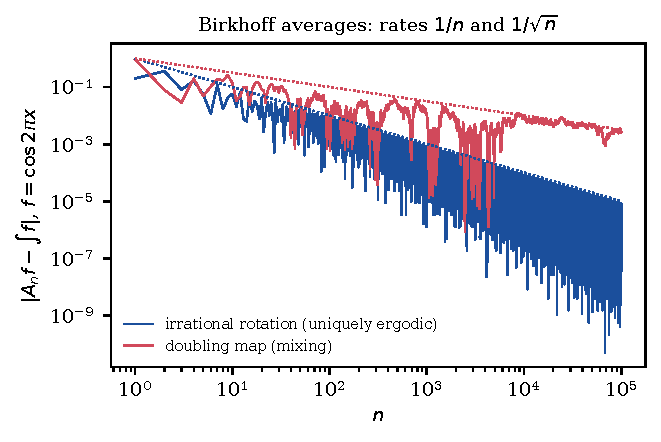
\includegraphics[width=0.85\textwidth]{birkhoff}
\caption{Birkhoff averages of $f(x)=\cos2\pi x$ along an orbit of the golden mean rotation, converging at rate $1/n$, and along an orbit of the doubling map, fluctuating at the central limit scale $1/\sqrt{n}$. The binary digits of the initial point of the doubling orbit are independent fair coin flips, and the orbit is computed as the shift of the digit sequence, each point being read from $52$ digits, because iterating $x\mapsto2x$ modulo one in floating point arithmetic reaches zero after $53$ steps. Dotted lines show the two rates.}
\label{fig:birkhoff}
\end{figure}

\section{Mixing}

\begin{definition}
A measure preserving system is mixing if $\mu(T^{-n}A\cap B)\to\mu(A)\mu(B)$ for all measurable $A,B$, equivalently $\langle U_T^nf,g\rangle\to\int f\dd\mu\int\bar g\dd\mu$ for all $f,g\in L^2$. It is weakly mixing if the convergence holds in Ces\`aro mean of absolute values.
\end{definition}

Mixing implies ergodicity: if $A$ is invariant, take $B = A$ to get $\mu(A) = \mu(A)^2$. The irrational rotation is ergodic but not mixing, since $U_T^ne_1 = e^{2\pi in\alpha}e_1$ does not tend to zero weakly.

\begin{theorem}[Koopman and von Neumann~\cite{koopmanvonneumann1932}]
\label{thm:koopman_vonneumann}
A measure preserving system is weakly mixing if and only if the Koopman operator has no eigenfunctions other than constants.
\end{theorem}

We quote the theorem without proof; see Walters~\cite{walters1982}. The rotation has eigenfunctions $e_m$ with eigenvalues $e^{2\pi im\alpha}$ and is the archetype of a system with pure point spectrum, meaning that the eigenfunctions span $L^2(\mu)$; the cat map has no eigenfunctions other than constants and is mixing.

\begin{theorem}[The cat map is mixing]
\label{thm:cat_map_mixing}
The automorphism $T(x,y) = (2x+y,x+y)$ of $\T^2$ is mixing for Lebesgue measure.
\end{theorem}

\begin{proof}
Let $A = \begin{pmatrix}2&1\\1&1\end{pmatrix}$ and, for $k\in\Z^2$, $e_k(z) = e^{2\pi ik\cdot z}$. Then $e_k\circ T = e_{A^\top k}$, so $\langle U_T^ne_k,e_l\rangle = \mathbb{1}\{(A^\top)^nk = l\}$. The matrix $A^\top = A$ has eigenvalues $\lambda^{\pm1}$ with $\lambda = \frac{3+\sqrt5}{2}$, and its stable eigenvector has irrational slope, so no nonzero integer vector lies in the stable direction. Hence for $k\neq0$ the component of $k$ along the unstable eigenvector is nonzero and $|A^nk|\to\infty$, so $\langle U_T^ne_k,e_l\rangle = 0$ for $n$ large. This proves mixing for trigonometric polynomials, and density in $L^2$ together with $\|U_T^n\| = 1$ extends it to all $f,g$.
\end{proof}

Figure~\ref{fig:cat} shows the cat map acting on a colored image discretized on a $101\times101$ grid. After a few iterations the image is mixed, as Theorem~\ref{thm:cat_map_mixing} predicts for the continuous system. But the discretized map $z\mapsto Az$ modulo $101$ is a permutation of the finite set $(\Z/101\Z)^2$, and a permutation of a finite set has finite order, which is Poincar\'e's recurrence theorem~\cite{poincare1890} in its simplest form. The image must therefore return exactly, and it does, at $n = 25$, the order of $A$ in $GL_2(\Z/101\Z)$. The figure is a picture of the Zermelo paradox~\cite{zermelo1896} of Chapter~\ref{ch:poincare}: mixing on short time scales, recurrence on long ones. The recurrence time is set by the arithmetic of the grid size $N$ and not by the number $N^2$ of cells: the period never exceeds $3N$~\cite{dysonfalk1992}. Kac's lemma (Theorem~\ref{thm:kac_lemma}) says that for an ergodic system the mean return time to a set of measure $1/N^2$ is $N^2$, and the discretized map is not ergodic. It splits the grid into cycles, here the fixed origin and $408$ cycles of length $25$, so the picture shows an artifact of the discretization and not the recurrence time of the continuous system.

\begin{figure}[t]
\centering
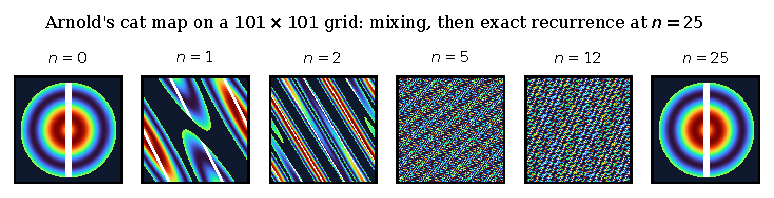
\includegraphics[width=\textwidth]{cat_map}
\caption{The cat map acting on an image on a $101\times101$ grid. The image is mixed within a few steps, and returns exactly after $25$ steps, the order of the cat map matrix modulo $101$. The discretized map is a permutation of the $101^2$ cells, and on an $N\times N$ grid its period never exceeds $3N$.}
\label{fig:cat}
\end{figure}

\section{Kolmogorov Sinai entropy}

Let $\xi = \{C_1,\dots,C_m\}$ be a finite measurable partition. Its entropy is $H(\xi) = -\sum_i\mu(C_i)\log\mu(C_i)$, and the join $\xi^n = \xi\vee T^{-1}\xi\vee\cdots\vee T^{-(n-1)}\xi$ is the partition into sets of points with the same itinerary of length $n$. By subadditivity of entropy the limit
\[
h(T,\xi) = \lim_{n\to\infty}\frac1nH(\xi^n)
\]
exists, and the Kolmogorov Sinai entropy~\cite{kolmogorov1958,sinai1959} is $h(T) = \sup_\xi h(T,\xi)$. It is an isomorphism invariant: isomorphic systems have equal entropy.

\begin{theorem}[Kolmogorov, Sinai~\cite{kolmogorov1959,sinai1959}]
\label{thm:kolmogorov_sinai}
Call a finite partition $\xi$ generating if the partitions $T^{-k}\xi$ generate $\mathcal{B}$ up to null sets, where $k$ ranges over $\Z$ if $T$ is invertible and over $k\geq0$ if it is not. If $\xi$ is generating, then $h(T) = h(T,\xi)$.
\end{theorem}

We quote the theorem without proof; see Walters~\cite[Chapter~4]{walters1982}.

\begin{example}[Entropy computations]
\begin{enumerate}
\item For the Bernoulli shift with marginal $p$, the time zero partition is generating and $\xi^n$ consists of cylinder sets with independent coordinates, so $H(\xi^n) = nH(p)$ and $h = H(p)$. Two Bernoulli shifts with different entropies are therefore not isomorphic, which answered the question of von Neumann~\cite{vonneumann1932operator} whether the shifts on two and three symbols with uniform weights are isomorphic: their entropies are $\log2$ and $\log3$.
\item For an irrational rotation, the partition into two arcs is generating, and $\xi^n$ has at most $2n$ atoms, since $n$ rotated copies of two endpoints cut the circle into at most $2n$ arcs. Hence $h\leq\lim\frac1n\log(2n) = 0$.
\item For the cat map, $h = \log\lambda = \log\frac{3+\sqrt5}{2}$, which also follows from Pesin's formula in Section~\ref{sec:lyapunov_logistic} because Lebesgue measure is invariant. More generally a toral automorphism has entropy $\sum\log|\lambda_i|$ over eigenvalues of modulus greater than one~\cite{yuzvinskii1967}; see also Walters~\cite{walters1982}.
\end{enumerate}
\end{example}

\begin{theorem}[Shannon, McMillan and Breiman~\cite{shannon1948,mcmillan1953,breiman1957}]
\label{thm:shannon_mcmillan_breiman}
Let $T$ be ergodic and $\xi$ a finite partition. Let $\xi^n(x)$ denote the atom of $\xi^n$ containing $x$. Then
\[
-\frac1n\log\mu\big(\xi^n(x)\big)\longrightarrow h(T,\xi)\qquad\text{almost surely and in }L^1.
\]
\end{theorem}

The theorem is the asymptotic equipartition property of information theory: typical itineraries of length $n$ have probability about $e^{-nh}$ and there are about $e^{nh}$ of them. We quote it without proof; see Cover and Thomas~\cite[Chapter~16]{covertomas}. For independent sequences it is the law of large numbers for $-\frac1n\sum\log p(X_i)$, and it is the dynamical form of the type counting of Chapter~\ref{ch:types}. Boltzmann's $S = k_B\log W$ and the Kolmogorov Sinai entropy, the growth rate of the number of distinguishable trajectories, are two counts of the same kind: one over configurations, the other over histories.

\begin{theorem}[Ornstein~\cite{ornstein1970}]
\label{thm:ornstein_isomorphism}
Two Bernoulli shifts on finite alphabets, indexed by $\Z$, are isomorphic if and only if they have the same entropy.
\end{theorem}

Ornstein's theorem of 1970 makes entropy a complete invariant within the Bernoulli class, and we quote it without proof. Many systems of physical interest are Bernoulli: ergodic toral automorphisms, among them the cat map~\cite{katznelson1971}, Sinai billiards~\cite{gallavottiornstein1974} and geodesic flows on surfaces of negative curvature~\cite{ornsteinweiss1973}. In these systems, at the level of measure theory, deterministic dynamics is indistinguishable from a Bernoulli shift of the same entropy.

\section{Lyapunov exponents and the logistic map}\label{sec:lyapunov_logistic}

Let $T$ be a differentiable map of an interval and $\mu$ an ergodic invariant probability measure for which $\log|T'|$ is integrable. The Lyapunov exponent is $\chi = \int\log|T'|\dd\mu$, and Birkhoff's theorem (Theorem~\ref{thm:birkhoff}) applied to $\log|T'|$ gives $\frac1n\log|(T^n)'(x)| = \frac1n\sum_{k<n}\log|T'(T^kx)|\to\chi$ for $\mu$ almost every $x$. Pesin's formula states that for a $C^2$ diffeomorphism of a compact manifold and an invariant measure absolutely continuous with respect to volume, the Kolmogorov Sinai entropy equals the integral of the sum of the positive Lyapunov exponents~\cite{pesin1977}. For absolutely continuous invariant measures of positive entropy of an interval map the corresponding statement is due to Ledrappier~\cite{ledrappier1981}. The logistic family is $T_r(x) = rx(1-x)$.

\begin{proposition}
\label{prop:logistic_r4}
For $r = 4$ the logistic map $T_4$ has the invariant density
\[
\rho(x) = \frac{1}{\pi\sqrt{x(1-x)}}
\]
on $(0,1)$. It is ergodic for $\rho$ and conjugate to the tent map, and its Lyapunov exponent and entropy with respect to $\rho$ are both $\log2$.
\end{proposition}

\begin{proof}
Let $\Lambda(y) = 1-|1-2y|$ be the tent map on $[0,1]$ and $\psi(y) = \sin^2(\pi y/2)$, an increasing homeomorphism of $[0,1]$ with $\psi'(y) = \frac\pi2\sin(\pi y)>0$ on $(0,1)$. Since $4\sin^2a\cos^2a = \sin^2(2a)$ we have $T_4(\psi(y)) = \sin^2(\pi y)$, and $\sin^2(\pi y) = \psi(\Lambda(y))$ because $\Lambda(y) = 2y$ for $y\leq\frac12$ and $\Lambda(y) = 2-2y$ for $y\geq\frac12$. Hence $T_4\circ\psi = \psi\circ\Lambda$, so $T_4$ is conjugate to the tent map. The tent map preserves Lebesgue measure, because every interval has two preimages of half its length. The image of Lebesgue measure under $\psi$ has density $\rho$, because $\psi^{-1}(x) = \frac2\pi\arcsin\sqrt x$ has derivative $\rho(x)$, so $\rho$ is invariant for $T_4$.

Let $b_1,b_2,\dots$ be the binary digits of $y$ and let $c_n = 1$ if $\Lambda^{n-1}(y)\geq\frac12$ and $c_n = 0$ otherwise. Then $c_1 = b_1$ and $c_n = b_n+b_{n-1}\pmod 2$ for $n\geq2$, because $\Lambda$ acts on a point with first digit $b_1$ by shifting the digits and, when $b_1 = 1$, complementing them. The map $(b_n)\mapsto(c_n)$ is a bijection of $\{0,1\}^{\mathbb{N}}$ that preserves the fair coin measure, since it is a bijection of $\{0,1\}^n$ on the first $n$ coordinates for every $n$. For Lebesgue distributed $y$ the digits $b_n$ are fair coin flips, so the itinerary $(c_n)$ of $y$ with respect to $[0,\frac12]$ and $[\frac12,1]$ is a sequence of fair coin flips, and $\Lambda$ acts on itineraries as the shift. Thus $\Lambda$ is isomorphic to the one sided fair coin shift. It follows that $\Lambda$ is ergodic for Lebesgue measure and $T_4$ is ergodic for $\rho$. The itinerary determines $y$, so the partition at $\frac12$ is a one sided generator with $H(\xi^n) = n\log2$, and Theorem~\ref{thm:kolmogorov_sinai} gives $h(\Lambda) = \log2$. Isomorphic systems have equal entropy, so $T_4$ has entropy $\log2$ for $\rho$.

For the exponent, differentiate $T_4\circ\psi = \psi\circ\Lambda$ at $y\neq\frac12$, using $|\Lambda'| = 2$, to get
\[
\log|T_4'(\psi(y))| = \log2+\ell(\Lambda(y))-\ell(y),
\]
where $\ell(y) = \log\psi'(y) = \log\frac\pi2+\log\sin(\pi y)$. The function $\ell$ is integrable on $[0,1]$, since $\log\sin(\pi y)$ has only logarithmic singularities at the endpoints. Integrate over $y$ with respect to Lebesgue measure. Because $\Lambda$ preserves it, $\int\ell\circ\Lambda\dd y = \int\ell\dd y$, and because $\psi$ carries it to $\rho(x)\dd x$ we obtain $\int\log|T_4'|\rho\dd x = \log2$. So $\log|T_4'|$ is integrable for $\rho$, although $T_4'$ vanishes at $x = \frac12$, and $\chi = \log2$. The entropy equals $\chi$, in agreement with the entropy formula for interval maps.
\end{proof}

The invariant density is the arcsine law, the Beta$(\frac12,\frac12)$ distribution. It is L\'evy's law of the time that Brownian motion spends positive (Chapter~\ref{ch:brownian}) and the law of the horseshoe shrinkage coefficient (Chapter~\ref{ch:mixtures}). Ulam and von Neumann proposed iterating this map as a generator of random numbers~\cite{ulamvonneumann1947}. Figure~\ref{fig:logistic} shows the attractor of the logistic family as $r$ varies, colored by the numerically computed Lyapunov exponent. Periodic windows, where the exponent is negative and the attractor is a finite cycle, alternate with chaotic parameter sets of positive Lebesgue measure, a theorem of Jakobson~\cite{jakobson1981}; Lyubich proved that for almost every parameter the map is either regular or stochastic~\cite{lyubich2002}.

\begin{figure}[t]
\centering
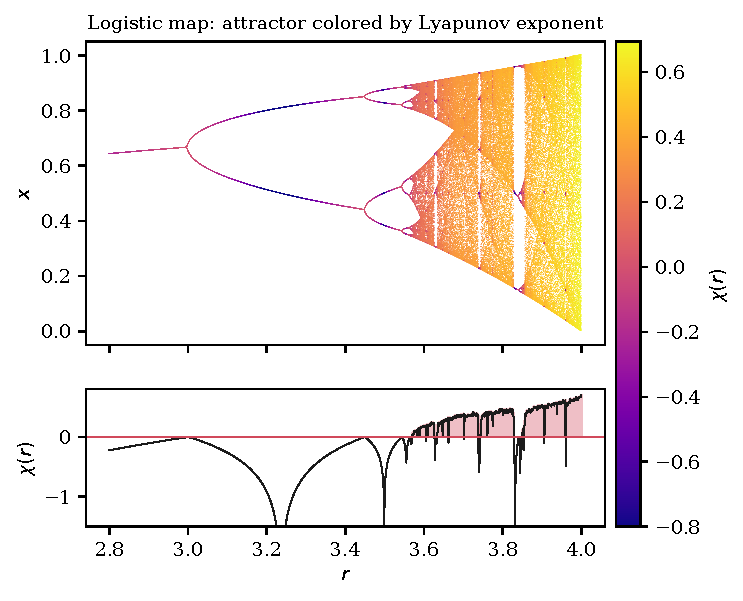
\includegraphics[width=0.85\textwidth]{logistic}
\caption{The logistic map $x\mapsto rx(1-x)$ for $1600$ values of $r$ from $2.8$ to $4$. Top, the attractor, drawn from the last $150$ of $400$ iterates that follow $600$ discarded ones, colored by the Lyapunov exponent with the color scale clipped to the interval from $-0.8$ to $0.7$. Bottom, the exponent, estimated as the average of $\log|r(1-2x_k)|$ over the $400$ iterates, positive (shaded) on chaotic parameters and negative in periodic windows; the vertical axis is cut at $-1.5$.}
\label{fig:logistic}
\end{figure}

\section{KAM theory and the failure of ergodicity}

Kolmogorov announced in 1954~\cite{kolmogorov1954}, and Arnold~\cite{arnold1963} and Moser~\cite{moser1962} proved in the early 1960s, that for a small perturbation of an integrable Hamiltonian system satisfying a nondegeneracy condition, most invariant tori survive, deformed but intact, and fill a set of positive measure. On each surviving torus the motion is quasiperiodic, and the energy surface is not ergodic. Markus and Meyer showed in 1974~\cite{markusmeyer1974} that generic Hamiltonian systems are neither integrable nor ergodic. The standard map of Chirikov~\cite{chirikov1979}
\[
p_{n+1} = p_n+K\sin q_n,\qquad q_{n+1} = q_n+p_{n+1}\pmod{2\pi}
\]
is the simplest model. Figure~\ref{fig:standard} shows orbits at the parameter at which, according to Greene's criterion~\cite{greene1979}, the last invariant circle spanning the cylinder breaks. Invariant curves, chains of islands around periodic orbits, and a chaotic sea coexist, as they do in the H\'enon Heiles system of Figure~\ref{fig:hh}. Ergodicity fails for typical Hamiltonian systems with few degrees of freedom, and Boltzmann's hypothesis cannot be the foundation of statistical mechanics for them.

\begin{figure}[t]
\centering
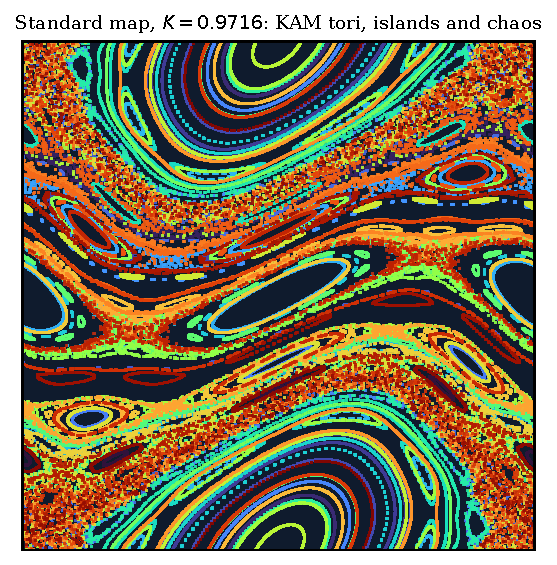
\includegraphics[width=0.78\textwidth]{standard_map}
\caption{Ninety orbits of the Chirikov standard map at $K = 0.971635$, near the breakup of the last spanning invariant circle, each in its own color: invariant curves, island chains and a chaotic sea. Each orbit has $900$ points, and the initial points are drawn uniformly from $[0,2\pi)^2$ with a fixed random seed.}
\label{fig:standard}
\end{figure}

\section{Khinchin's argument}

Khinchin's \emph{Mathematical Foundations of Statistical Mechanics}, published in Russian in 1943 and in English in 1949~\cite{khinchin1949}, replaced ergodicity by concentration. Consider $n$ particles with phase point $z = (z_1,\dots,z_n)$ on an energy surface, a Hamiltonian $H(z) = \sum_iH_i(z_i)$ that is a sum of one particle terms, and a sum function $F(z) = \sum_if_i(z_i)$, the form of macroscopic observables such as pressure or kinetic energy, with summands $f_i$ bounded independently of $n$ and a microcanonical mean $m$ of order $n$. Khinchin showed that the standard deviation $s$ of $F$ for the microcanonical measure is of order $n^{1/2}$. Markov's inequality gives $\P(|F-m|\geq am)\leq s/(am)$, which is of order $n^{-1/2}/a$, so the set where the relative deviation of $F$ exceeds $k_1n^{-1/4}$ has microcanonical measure at most $k_2n^{-1/4}$, with $k_1$ and $k_2$ independent of $n$. The mean ergodic theorem, which needs no ergodicity, carries the bound over to time averages. Let $T$ be the time one map of the Hamiltonian flow, which preserves the microcanonical measure. By Theorem~\ref{thm:vonneumann} the averages $\frac1N\sum_{k<N}F\circ T^k$ converge in $L^2$, as $N\to\infty$ at fixed $n$, to $\E[F\mid\mathcal{I}]$, the conditional expectation given the invariant $\sigma$ algebra. This limit has the same mean as $F$ and a variance no larger than that of $F$, because conditional expectation is an orthogonal projection in $L^2$, so Markov's inequality gives it the same bound. Hence, whatever the ergodic properties of the dynamics, the infinite time average of $F$ differs from its phase average by less than the fraction $k_1n^{-1/4}$ of the phase average except on a set of initial conditions of measure at most $k_2n^{-1/4}$. This is Khinchin's theorem, which Mazur and van der Linden extended to particles with short range interactions~\cite{mazurvanderlinden1963}. The argument is the one we use in Chapter~\ref{ch:entropy} to explain why macroscopic observables are deterministic: Lipschitz functions of many weakly dependent coordinates concentrate. In this sense the sixth problem needs less than ergodicity and more than it: less, because concentration suffices for equilibrium averages; more, because the approach to equilibrium on physical time scales is a statement about the dynamics of the one particle law, the subject of Lanford's theorem~\cite{lanford1975} in Chapter~\ref{ch:kinetic}, and not about infinite time averages.

\section{The ergodic decomposition and de Finetti}

The set of $T$ invariant probability measures is convex and, for a continuous map of a compact metric space, weakly compact. Its extreme points are exactly the ergodic measures: if $\mu = t\mu_1+(1-t)\mu_2$ nontrivially and $A$ is invariant with $0<\mu(A)<1$, then $\mu(\cdot\mid A)$ and $\mu(\cdot\mid A^c)$ give such a decomposition, and conversely. This set is moreover a Choquet simplex, a compact convex set in which every point is the barycenter of a unique probability measure on the extreme points~\cite{phelps2001}, so Choquet theory gives the ergodic decomposition: every invariant measure is a unique mixture of ergodic ones,
\[
\mu = \int\mu_\theta\,\Pi(\dd\theta),
\]
where $\theta$ labels the ergodic measures and $\mu_\theta$ is the conditional measure of $\mu$ given the invariant $\sigma$ algebra, obtained by disintegration; see Walters~\cite{walters1982}. De Finetti's theorem (Theorem~\ref{thm:definetti}) is the ergodic decomposition for the group of finite permutations acting on sequences: the invariant measures are exchangeable laws, the ergodic ones are, by the Hewitt Savage zero one law~\cite{hewittsavage1955}, the independent identically distributed laws, and the mixing measure $\Pi$ is the prior; see Kallenberg~\cite{kallenberg2005}. Birkhoff's theorem says that the empirical frequencies along a single orbit identify the ergodic component, so that the parameter $\theta$ is a function of the whole sequence, and the martingale convergence theorem then gives $\E[g(\theta)\mid X_1,\dots,X_n]\to g(\theta)$ almost surely for bounded $g$. This is the statement that the posterior concentrates on the true parameter, Doob's theorem~\cite{doob1949} (Theorem~\ref{thm:doob}) seen through the ergodic decomposition.

\section{Markov chains, spectral gaps and Monte Carlo}\label{sec:markov_spectral_mc}

A Markov kernel $P$ is reversible with respect to $\pi$ if $\pi(\dd x)P(x,\dd y) = \pi(\dd y)P(y,\dd x)$, and then $\pi$ is invariant for $P$. The stationary chain is a stationary process, and if the chain is irreducible, meaning that every $P$ invariant set has $\pi$ measure zero or one, the shift on path space is ergodic. Birkhoff's theorem (Theorem~\ref{thm:birkhoff}) applied to the shift gives $\frac1n\sum_{k<n}f(X_k)\to\int f\dd\pi$ almost surely for $f\in L^1(\pi)$ and $\pi$ almost every starting point. Its quantitative form is a central limit theorem.

\begin{theorem}[Kipnis and Varadhan~\cite{kipnisvaradhan1986}]
\label{thm:kipnis_varadhan}
Let $P$ be reversible with respect to $\pi$ and aperiodic, with spectrum in $[-1,1-g]$ on mean zero functions, $g>0$. For $f\in L^2(\pi)$ with $\int f\dd\pi = 0$, the stationary chain satisfies $\frac{1}{\sqrt n}\sum_{k<n}f(X_k)\to N(0,\sigma_f^2)$ in law, with
\[
\sigma_f^2 = \big\langle f,(I+P)(I-P)^{-1}f\big\rangle_\pi\leq\frac{2-g}{g}\,\Var_\pi(f).
\]
\end{theorem}

We quote the central limit theorem without proof; see Roberts and Rosenthal~\cite{robertsrosenthal2004} for the statement for chains in discrete time.

\begin{proof}[Proof of the variance bound]
By the spectral theorem, $\sigma_f^2 = \int\frac{1+s}{1-s}\,\nu_f(\dd s)$ where $\nu_f$ is the spectral measure of $f$, supported in $[-1,1-g]$ with total mass $\Var_\pi(f)$. The function $s\mapsto\frac{1+s}{1-s}$ is increasing, so it is at most $\frac{2-g}{g}$ on the support.
\end{proof}

The spectral gap $g$ is a Poincar\'e constant in the sense of Chapter~\ref{ch:poincare}, and the asymptotic variance of a Monte Carlo average is the integrated autocorrelation of the chain. Every Markov chain Monte Carlo computation in this book, from the Gibbs samplers of P\'olya Gamma augmentation in Chapter~\ref{ch:mixtures} to the preconditioned Crank Nicolson sampler for Navier Stokes posteriors in Chapter~\ref{ch:nsinference}, is an application of the ergodic theorem, and for the reversible samplers among them the cost is governed by a spectral gap. The preconditioned Crank Nicolson proposal is reversible with respect to the Gaussian prior, so the Metropolis accept step makes the chain reversible with respect to the posterior~\cite{cotter2013}. A Gibbs sampler that alternates between two blocks $u$ and $v$ is not reversible as a chain on the pair, but its marginal chain on $u$ is: with $K(u,\dd u') = \int p(\dd v\mid u)\,p(\dd u'\mid v)$ and $\pi$ the marginal law of $u$, we have $\pi(\dd u)K(u,\dd u') = \int p(\dd v)\,p(\dd u\mid v)\,p(\dd u'\mid v)$, which is symmetric in $u$ and $u'$. The physicists of Los Alamos who invented the Metropolis algorithm~\cite{metropolis1953} were, in this precise sense, building an ergodic system on purpose.

\section*{Notes}

Walters's \emph{Introduction to Ergodic Theory}~\cite{walters1982} and Petersen's \emph{Ergodic Theory}~\cite{petersen1983} cover the material of this chapter, and Arnold and Avez~\cite{arnoldavez1968} treat the cat map and the other classical examples. The ergodic decomposition view of de Finetti's theorem is developed by Kallenberg in \emph{Probabilistic Symmetries and Invariance Principles}~\cite{kallenberg2005}.

\section*{Exercises}
\begin{enumerate}
\item Show that the doubling map is mixing by computing $\langle U_T^ne_k,e_l\rangle$.
\item Let $T$ be the cat map and $\lambda = \frac{3+\sqrt5}{2}$. Show that $T^n$ has exactly $\lambda^n+\lambda^{-n}-2$ fixed points on $\T^2$, and that their exponential growth rate is the entropy $h(T)$.
\item For the doubling map $T$ and $f(x) = \cos2\pi x$, show that the functions $f\circ T^k$, $k\geq0$, are orthogonal in $L^2$ and that $\E[f\mid T^{-1}\mathcal{B}] = 0$. Deduce that the Birkhoff average $A_nf$ has variance exactly $1/(2n)$, and that $\sqrt nA_nf$ converges in law to $N(0,\frac12)$ by the martingale central limit theorem.
\item For the golden mean $\alpha$, show that $|\sin\pi m\alpha|\geq c/m$ for some $c>0$ and all $m\geq1$. Deduce that for the rotation by $\alpha$ the Birkhoff averages of every $f$ with $\sum_m|m||\hat f(m)|<\infty$ converge to $\int f$ at the rate $O(1/n)$.
\item Let $P$ be the transition matrix of the chain on $\{-1,+1\}$ that changes state with probability $p\in(0,1)$. For $f(x) = x$, compute the spectral gap and the asymptotic variance of $\frac{1}{\sqrt n}\sum_{k<n}f(X_k)$, and decide whether the bound of Theorem~\ref{thm:kipnis_varadhan} is attained.
\item Show that the period of the cat map on an $N\times N$ grid equals the order of $A$ in $GL_2(\Z/N\Z)$, and compute it for $N = 101$. Compare the cycle lengths with the mean return time that Kac's lemma (Theorem~\ref{thm:kac_lemma}) gives for an ergodic system on $N^2$ cells.
\end{enumerate}
